\documentclass[aspectratio=43]{beamer}
% Theme works only with a 4:3 aspect ratio
\usetheme{CSCS}

\usepackage{tikz}
\usepackage{pgfplots}
\usepackage{pgfplotstable}
\usetikzlibrary{pgfplots.groupplots,spy,patterns}
\usepackage{listings}
\usepackage{color}
\usepackage{tcolorbox}
\usepackage{anyfontsize}
\usepackage{xspace}
\usepackage{graphicx}

% define footer text
\newcommand{\footlinetext}{Introduction to GPUs in HPC}

% Select the image for the title page
\newcommand{\picturetitle}{cscs_images/image5.pdf}

% fonts for maths
\usefonttheme{professionalfonts}
\usefonttheme{serif}

% source code listing
\newcommand{\axpy}{{\ttfamily axpy}\xspace}

% set indent to a more reasonable level (so that itemize can be used in columns)
\setlength{\leftmargini}{20pt}

\DeclareTextFontCommand{\emph}{\bfseries\color{blue!70!black}}

% Please use the predifined colors:
% cscsred, cscsgrey, cscsgreen, cscsblue, cscsbrown, cscspurple, cscsyellow, cscsblack, cscswhite

\author{Ben Cumming, CSCS}
\title{Introduction to GPUs in HPC}
\subtitle{}
\date{\today}

\begin{document}

% TITLE SLIDE
\cscstitle

%++++++++++++++++++++++++++++++++
\cscschapter{Using MPI with GPUs}
%++++++++++++++++++++++++++++++++

%%%%%%%%%%%%%%%%%%%%%%%%%%%%%%%%%%%%%%%%%%%%
\begin{frame}[fragile]{What is MPI}
%%%%%%%%%%%%%%%%%%%%%%%%%%%%%%%%%%%%%%%%%%%%
    MPI (\emph{Message Passing Interface}) is a standardised library for message passing
    \begin{itemize}
        \item Highly portable: it is implemented on every HPC system available today.
        \item Has C, C++ and Fortran bindings.
        \item Supports point to point communication
        \begin{itemize}
            \item \lstterm{MPI_Send}, \lstterm{MPI_Recv}, \lstterm{MPI_Sendrecv}, etc.
        \end{itemize}
        \item Supports global collectives
        \begin{itemize}
            \item \lstterm{MPI_Barrier}, \lstterm{MPI_Gather}, \lstterm{MPI_Reduce}, etc.
        \end{itemize}
    \end{itemize}
    When you start an MPI application
    \begin{itemize}
        \item $N$ copies of the application are launched.
        \item Each copy is given a \emph{rank}$\in\{0,1,\dots,N-1\}$.
    \end{itemize}
\end{frame}

%%%%%%%%%%%%%%%%%%%%%%%%%%%%%%%%%%%%%%%%%%%%
\begin{frame}[fragile]{A basic MPI application}
%%%%%%%%%%%%%%%%%%%%%%%%%%%%%%%%%%%%%%%%%%%%
    \begin{code}{Example MPI application myapp.cpp}
        \begin{lstlisting}[style=boxcudatiny]
#include <mpi.h>
#include <unistd.h>
#include <cstdio>

int main(int argc, char** argv) {
    // initialize MPI on this rank
    MPI_Init(&argc, &argv);
    // get information about our place in the world
    int rank, size;
    MPI_Comm_rank(MPI_COMM_WORLD, &rank);
    MPI_Comm_size(MPI_COMM_WORLD, &size);
    // print a message
    char name[128]; gethostname(name, sizeof(name));
    printf("hello world from %d of %d on %s\n", rank, size, name);
    // close down MPI
    MPI_Finalize();
    return 0;
}
        \end{lstlisting}
    \end{code}

    MPI applications are compiled with a \emph{compiler wrapper}:
    \begin{terminal}{}
        \begin{lstlisting}[style=terminal]
> CC myapp.cpp -o myapp # the Cray C++ wrapper is CC
        \end{lstlisting}
    \end{terminal}
\end{frame}

%%%%%%%%%%%%%%%%%%%%%%%%%%%%%%%%%%%%%%%%%%%%
\begin{frame}[fragile]{Running our basic MPI application}
%%%%%%%%%%%%%%%%%%%%%%%%%%%%%%%%%%%%%%%%%%%%
    \begin{center}
        \begin{terminal}{}
            \begin{lstlisting}[style=terminal]
# run myapp 4 ranks (-n) on 4 nodes (-N)
> srun -n4 -N4 ./myapp
hello world from 0 of 4 on nid02117
hello world from 1 of 4 on nid02118
hello world from 2 of 4 on nid02119
hello world from 3 of 4 on nid02120
            \end{lstlisting}
        \end{terminal}

        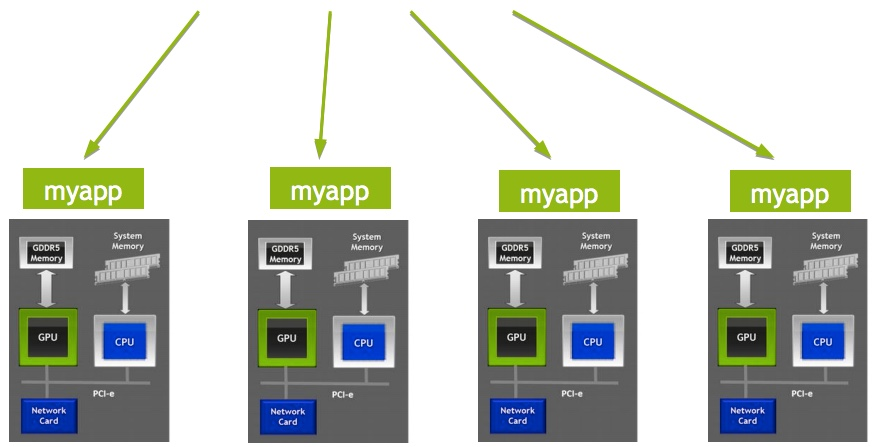
\includegraphics[width=0.8\textwidth]{./images/mpirun.jpg}
    \end{center}
    \footnotesize \quad\quad\quad\textcopyright NVIDIA Corporation
\end{frame}

%%%%%%%%%%%%%%%%%%%%%%%%%%%%%%%%%%%%%%%%%%%%
\begin{frame}[fragile]{MPI with data in device memory}
%%%%%%%%%%%%%%%%%%%%%%%%%%%%%%%%%%%%%%%%%%%%
    Use GPUs to parallelize on-node computation
    \begin{itemize}
        \item \dots and MPI for communication between nodes.
    \end{itemize}
    To use with data that is in buffers in GPU memory:
    \begin{enumerate}
        \item Allocate buffers in host memory;
        \item Manually copy from device$\rightarrow$host memory;
        \item Perform MPI communication with host buffers;
        \item Copy received data from host$\rightarrow$device memory.
    \end{enumerate}
    This approach can be very fast.
    \begin{itemize}
        \item Have a CPU thread dedicated to asynchronous host$\leftrightarrow$device and MPI communication
    \end{itemize}
\end{frame}

%%%%%%%%%%%%%%%%%%%%%%%%%%%%%%%%%%%%%%%%%%%%
\begin{frame}[fragile]{GPU-aware MPI}
%%%%%%%%%%%%%%%%%%%%%%%%%%%%%%%%%%%%%%%%%%%%
        GPU-aware MPI implementations can automatically handle MPI transactions with pointers to GPU memory
        \begin{itemize}
            \item MVAPICH 2.0
            \item OpenMPI since version 1.7.0
            \item Cray MPI
        \end{itemize}

    \begin{info}{How it works}
        \begin{itemize}
            \item Each pointer passed to MPI is checked to see if it is in host or device memory.
            If not set, MPI assumes that all pointers are to host memory, and your application will probably crash with segmentation faults
            \item Small messages between GPUs (up to $\approx$8 k) are copied directly with \emph{RDMA}
            \item Larger messages are \emph{pipelined} via host memory
        \end{itemize}
    \end{info}

\end{frame}

%%%%%%%%%%%%%%%%%%%%%%%%%%%%%%%%%%%%%%%%%%%%
\begin{frame}[fragile]{How to use G2G communication}
%%%%%%%%%%%%%%%%%%%%%%%%%%%%%%%%%%%%%%%%%%%%
    \begin{itemize}
        \item Set the environment variable \lst{export MPICH_RDMA_ENABLED_CUDA=1}
        \begin{itemize}
            \item If not set, MPI assumes that all pointers are to host memory, and your application will probably crash with segmentation faults
        \end{itemize}
        \item Experiment with the environment variable \lst{MPICH_G2G_PIPELINE}
        \begin{itemize}
            \item Sets the maximum number of 512 kB message chunks that can be in flight (default 16)
        \end{itemize}
    \end{itemize}

   \begin{code}{MPI with G2G example}
        \begin{lstlisting}[style=boxcudatiny]
MPI_Request srequest, rrequest;
auto send_data = malloc_device<double>(100);
auto recv_data = malloc_device<double>(100);

// call MPI with GPU pointers
MPI_Irecv(recv_data, 100, MPI_DOUBLE, source, tag, MPI_COMM_WORLD, &rrequest);
MPI_Isend(send_data, 100, MPI_DOUBLE, target, tag, MPI_COMM_WORLD, &srequest);
        \end{lstlisting}
   \end{code}

\end{frame}

%%%%%%%%%%%%%%%%%%%%%%%%%%%%%%%%%%%%%%%%%%%%
\begin{frame}[fragile]{Capabilities and Limitations}
%%%%%%%%%%%%%%%%%%%%%%%%%%%%%%%%%%%%%%%%%%%%
    \begin{itemize}
        \item Support for most MPI API calls (point-to-point, collectives, etc)
        \item Robust support for common MPI API calls
        \begin{itemize}
            \item i.e. point-to-point operations 
        \end{itemize}
        \item No support for user-defined MPI data types
    \end{itemize}
\end{frame}

%%%%%%%%%%%%%%%%%%%%%%%%%%%%%%%%%%%%%%%%%%%%
\begin{frame}[fragile]{Exercise: MPI with G2G}
%%%%%%%%%%%%%%%%%%%%%%%%%%%%%%%%%%%%%%%%%%%%
    \begin{itemize}
        \item 2D stencil with MPI in \lstterm{diffusion/diffusion2d_mpi.cu}
        \item Implement the G2G version
        \begin{enumerate}
            \item can you observe any performance differences?
            \item why are we restricted to just 1 MPI rank per node?
        \end{enumerate}
        \item Implement a version that uses managed memory
        \begin{itemize}
            \item what happens if you don't set \lstterm{MPICH_RDMA_ENABLED_CUDA}?
        \end{itemize}
    \item \emph{Extra++:} find the nasty performance bug...
    \end{itemize}

    \begin{terminal}{}
        \begin{lstlisting}[style=terminal]
# load modules require to compile MPI
module swap PrgEnv-cray PrgEnv-gnu
module load cudatoolkit

# launch with 2 MPI ranks
MPICH_RDMA_ENABLED_CUDA=1 srun -C gpu -n2 -N2 --reservation=summer
        diffusion2d_mpi.cuda 8

# plot the solution
source ../../../../scripts/plot.sh

# once it gets the correct results:
sbatch job.batch
        \end{lstlisting}
   \end{terminal}

\end{frame}

%%%%%%%%%%%%%%%%%%%%%%%%%%%%%%%%%%%%%%%%%%%%
\begin{frame}[fragile]{Exercises: 2D Diffusion with MPI Results}
%%%%%%%%%%%%%%%%%%%%%%%%%%%%%%%%%%%%%%%%%%%%
    \begin{info}{Time for 10,000 time steps \@ 128$\times$131,072 on P100 GPUs}
       \begin{center}
           \begin{tabular}{ccc}
               \hline
               nodes   &   G2G off & G2G on \\
                \hline
               1       &  5.579    &  5.580 \\
               2       &  3.083    &  2.811 \\
               4       &  1.909    &  1.426 \\
               8       &  1.203    &  0.737 \\
              16       &  0.836    &  0.399 \\
           \end{tabular}
       \end{center}
   \end{info}
\end{frame}

%%%%%%%%%%%%%%%%%%%%%%%%%%%%%%%%%%%%%%%%%%%%
\begin{frame}[fragile]{Using Unified Memory with MPI}
%%%%%%%%%%%%%%%%%%%%%%%%%%%%%%%%%%%%%%%%%%%%
    \begin{itemize}
        \item To pass a managed pointer to MPI you must use a GPU-aware MPI distribution.
        \item Even if the managed memory is on the host at time of calling.
    \end{itemize}

    \begin{columns}[T]
        \begin{column}{0.5\textwidth}
            \begin{itemize}
                \item The MPI implementation uses page-locked (pinned) memory for RDMA.
                \item If not aware of unified memory you get
                \begin{itemize}
                    \item if lucky: crashes.
                    \item if unlucky: infuriating bugs.
                \end{itemize}
            \end{itemize}
        \end{column}

        \begin{column}{0.5\textwidth}
            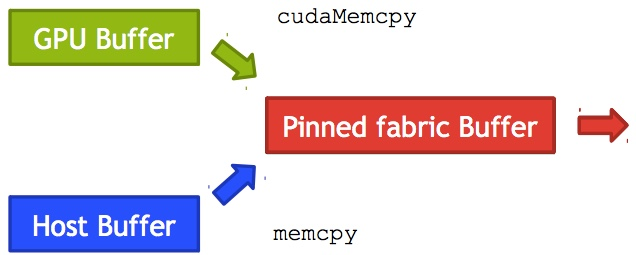
\includegraphics[width=\textwidth]{./images/rdmacopy.jpg}\\
            \footnotesize \textcopyright NVIDIA Corporation
        \end{column}
    \end{columns}
\end{frame}

\end{document}
